\chapter{Implementation Framework for an energy trading platform using blockchain technology} \label{framework}
\label{chapter4}
In this chapter we go through our proposed energy trading architecture. We analyze the layers of our implementation and
discuss about the different aspects of our solution like the network roles, the network tokens and their minting and burning mechanism and finally we mention
possible integration solutions with other networks.

\section{Overview}
After reviewing the current literature in regards to energy trading using blockchain technology, we introduce a novel energy trading platform that tries
to improve upon the existing implementation. The main limitation we identified with the existing energy trading platforms is the need for an efficient energy
generation and consumption forecast. Most prosumers make use of renewable energy generation units like PV panels which are very sensitive to weather conditions.
This makes it very challenging to produce good energy generation predictions which can cause issues with a direct energy trading approach. The actual energy
generated during the energy consumption period might be less than the energy trading agreement made with a consumer during the trading period. This causes the need
for the microgrid to be connected to the main grid to buy any extra energy need or even sell any excess energy that was not actually consumed.
The model we will introduce in the next sections relies on an indirect energy trading paradigm and introduces the role of storage provider in the microgrid.
This new role will be responsible to store the energy produced by the network.\\
The main challenges we are trying to address with our proposed model are the following:
\begin{itemize}
    \item \textbf{Decentralization}: We want the network to be autonomous and capable of operating by its own with no intermediates. No single authority should
          should be able to control the network's energy market prices which should only be influence by the network's energy trading needs.
    \item \textbf{Autonomy}: We want to create a model which can be as autonomous as possible with minimal energy trading transactions with the main energy grid.
    \item \textbf{Forecasting Errors}: We want to minimize any energy generation and consumption forecasting errors as much as possible to avoid any breach in energy
          trading agreements.
    \item \textbf{Fault Tolerance}: We need to create an architecture which is tolerant in energy storing and delivering failures.
\end{itemize}
We call our proposed energy trading platform "PowerChain" and we will refer to it as such in the following sections.

\section{PowerChain Components}

PowerChain consists of two main layers:
\begin{itemize}
    \item The \textbf{Blockchain Layer}: It is responsible for the digitalization and transferring of energy produced by the network.
    \item And the \textbf{Market Layer}: It is responsible for the trading of digital energy assets with legal currencies.
\end{itemize}

These two layers are completely separate from each other and could potentially operate separately by themselves.
The blockchain layer is used to digitize the available energy and makes it possible to transfer the energy assets while the market layer is used to
trade the digitized energy assets for legal currencies with the only link between them being the digitized energy assets.
In the following chapters more details will be presented for the different aspects of PowerChain.

\pagebreak

\subsection{PowerChain Layers}
PowerChain defines two different type of main layers, the physical layers and the information layers. The information layer works on top of the physical layer and its
responsibility is to orchestrate energy consumption, production and storage. The physical layer consists of the energy storage batteries, the energy production units 
and the energy consumers. We recognize three physical layers and two information layers which are analyzed below.\\

\begin{figure}[h!]
    \centering
    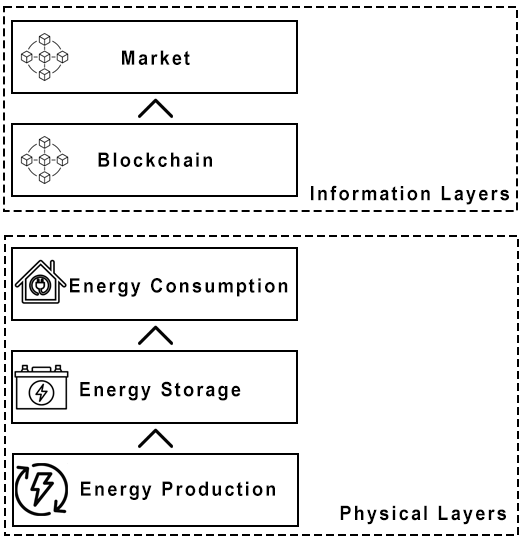
\includegraphics[scale=0.6]{Figures/PowerChain_Layers.png}
    \caption{PowerChain Layers}
\end{figure}

\textbf{Physical Layers:}
\begin{itemize}
    \item \textbf{Production Layer}: This layer consists of all the energy production units that exist in the microgrid. It's a very crucial layer of the architecture as it
          produces the network's energy.
    \item \textbf{Storage Layer}: This layer is comprised by all the energy storage units of the microgrid. The energy produced by the production layer is stored in the storage
          layer for later consumption.
    \item \textbf{Consumption Layer}: It is made of all the peers that consume energy from the storage layer.
\end{itemize}

\textbf{Information Layers:}
\begin{itemize}
    \item \textbf{Blockchain Layer}: The blockchain layer is the heart of the PowerChain protocol. It facilitates all the necessary functionality to digitize the produced energy and
          make it tradable through smart contracts.
    \item \textbf{Market Layer}: In the market layer, the digitized energy is getting traded between the peers. This layer could be completely separated from the blockchain layer. It consists
          of all the possible ways the digitized energy could be traded. PowerChain provides also a market platform that can be used to initiate trades.
\end{itemize}

\subsection{Network Roles}
In literature, two roles are usually defined in an energy trading network, the consumer and the consumer/producer called prosumer.
Apart from the roles of energy producer and consumer we also define the role of energy storage provider. In more detail:
\begin{itemize}
    \item \textbf{The consumer}, is buying and consuming the available energy of the network which is stored by the storage providers.
    \item \textbf{The producer}, is producing network's energy using energy generation units like PVs. The produced energy is send to the storage providers for storage.
    \item \textbf{The storage providers}, are receiving the energy from producers and they are storing it in batteries.
\end{itemize}
\begin{figure}[h!]
    \centering
    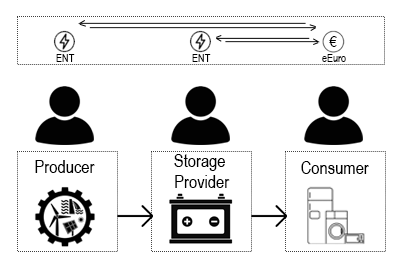
\includegraphics[scale=0.6]{Figures/powerchain_scheme.png}
    \caption{PowerChain energy exchange diagram}
\end{figure}
Each network participant can have one or multiple of these three roles. Every time a producer is storing energy in the batteries of a storage provider, the storage provider is getting
a percentage of the gains. The gains are in the form of digital energy tokens, called ENT tokens, described in more detail in the following chapter. \\

\subsection{Network Tokens}
PowerChain defines two different type of tokens in the network:
\begin{itemize}
    \item \textbf{Energy Token}: The energy token is a token backed by the Network's stored energy. A single energy token corresponds to specific kilowatt-hours (kWh) of energy. It digitizes the energy of the network and thus making 
    it exchangeable and transactable. It is the heart of the whole network as it represents the actual energy that is produced, consumed and transacted. To link the energy token value with the actual energy of the network, we make use of
    a token minting and burning mechanism, described in more details in the following section.
    \item \textbf{Currency Token}: The currency token is backed by a real work currency which could be for example Euro, Dollar, Pound or any other legal currency. One currency token corresponds to exactly one unit of the backed currency.
    The existence of a currency token, is important for the network in order to enable token exchanges. Energy producers that want to sell their energy, need to sell their energy tokens while energy consumers need to buy energy
    tokens to consume the corresponding energy. The currency token is what brings real world currencies into the network to make this exchange possible. In the following chapter we describe how to bridge a real world currency into the
    network.
\end{itemize}
For the purpose of this project, we will use Euro as the backed currency of currency token. For simplicity reasons we will call the Euro currency token as eEuro and the energy token as ENT.
In the following sections, more details are provided for the minting and burning of the mentioned tokens.\\

\subsubsection{Minting/Burning of ENT tokens}
ENT tokens are minted every time energy is stored in the storage layer. For every kWh of energy stored in the storage layer, an amount of ENT tokens are minted into the wallets of the producer and the storage provider. For every kWh consumed from the
storage layer, an amount of ENT is burned. The amount of ENT tokens minted or burned is determined by the PowerChain smart contract and is a function of the total ENT tokens in circulation and the total kWh of energy stored in the storage layer.
We define the minting and burning functions as follows:
\begin{empheq}[box=\fbox]{align}
            \textrm{ENT}_{mint} &=
            \left\{
            \begin{array}{ll}
                1 - R & \textrm{, When } R < M \\
                M                                          & \textrm{, Otherwise} \\
            \end{array}
            \right. \\ 
            \textrm{ENT}_{burn} &=
            \left\{
            \begin{array}{ll}
                1 + R & \textrm{, When } R < B \\
                B                                                                & \textrm{, Otherwise} \\               
            \end{array}
            \right. \\ 
            R &= |\textrm{KWH} - \textrm{ENT}| \times C   
\end{empheq}
Where,\\
\begin{tabular}{rl}
    $\textrm{ENT}_{mint}$ & :  ENT tokens to be minted per kWh produced. \\
    $\textrm{ENT}_{burn}$ & :  ENT tokens to be burned per kWh consumed.    \\
    $R$                   & :  The amount of ENT to be paid as cost for minting/burning ENT \\
                          &    for each kWh produced/consumed. \\
    $\textrm{KWH}$        & :  Total kWh stored in storage layer.       \\
    $\textrm{ENT}$        & :  Total ENT tokens in circulation.          \\
    $C$                   & :  A constant where $0<c<1$. Defines the percentage of energy loss \\ 
                          &    to be covered per kWh produced/consumed. \\
    $M$                   & :  The maximum ENT/kWh minting cost.          \\
    $B$                   & :  The maximum ENT/kWh burning cost.         \\
\end{tabular}\\

\begin{figure}[h!]
    \centering
    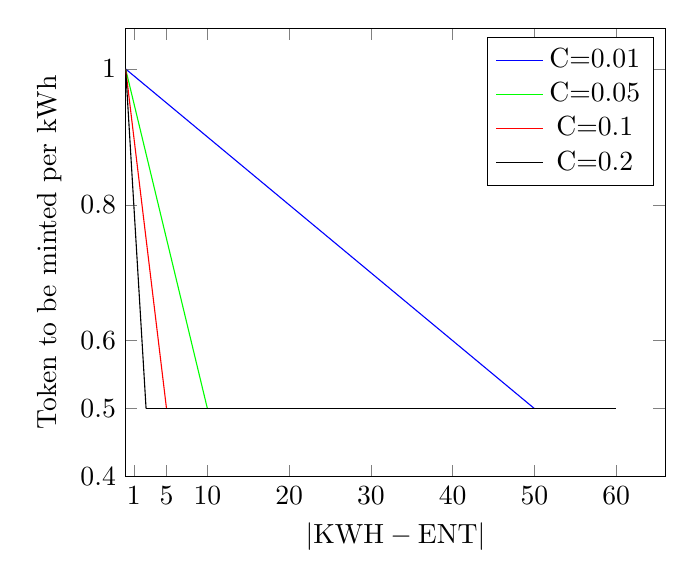
\begin{tikzpicture}
        \begin{axis}[ 
          xlabel=$|\textrm{KWH} - \textrm{ENT}|$,
          ylabel={Token to be minted per kWh},
          xtick={1,5,10,20,30,40,50,60},
          ytick={0,0.2,0.4,0.5,0.6,0.8,1},
          ymin = 0.4,
          xmin = 0
        ]
        \addplot[domain=0:50,color=blue] {1 - x * 0.01};
        \addlegendentry{C=0.01}
        \addplot[domain=0:10,color=green] {1 - x * 0.05};
        \addlegendentry{C=0.05}
        \addplot[domain=0:5,color=red]{1 - x * 0.1};
        \addlegendentry{C=0.1}
        \addplot[domain=0:2.5,color=black]{1 - x * 0.2};
        \addlegendentry{C=0.2}

        \addplot[domain=50:60,color=black]{0.5};
        \addplot[domain=10:60,color=black]{0.5};
        \addplot[domain=5:60,color=black]{0.5};
        \addplot[domain=2.5:60,color=black]{0.5};
        \end{axis}
      \end{tikzpicture}
    \caption{ENT Minting/burning cost for 1 kWh produced/consumed versus the difference between total kWh and total ENT in the network, for different values of C with M = B = 0.5 ENT/kWh}
\end{figure}

The reason we set a cost for minting and burning ENT tokens, is to try to keep the ratio between the total kWh and the total ENT in the network, to 1. Let's consider that for every produced kWh we mint 1 ENT token, in this situation for every $X$ kWh stored we will have $X$ amount of ENT tokens. 
The problem arises when we lose energy due to a potential battery disfunction. In such situation, we will have $Y<X$ kWh available while there are still $X$ amount of ENT tokens in circulation. By applying the minting and burning
functions mentioned above, more tokens will be burned per kWh spent and less tokens will be minted per kWh generated until an equilibrium is reached. This is achieved through the cost function R which adds a cost to every minting 
and burning of ENT tokens in order to keep the total kWh of the storage layer equal to the total ENT in circulation. The constant $C$, defines the percentage of the missing energy to be covered during minting or burning of tokens. The higher the value of the constant, 
the faster equilibrium will be reached but the higher the ENT cost for the individuals, meaning that in practice less network participants are going to cover the loss.\\
The issue with the above mentioned equations, is that we approach equilibrium asymptotically because on each step we cover a fraction of the difference and as we progress that fraction tends to zero. To reach equilibrium in a finite amount of steps and keep the energy loss cost distribution fair, 
the cost $R$ is calculated only when the difference between total kWh and total ENT tokens increase. This means that for every decrease of the difference between these two values, the $R$ value will remain the same until equilibrium is reached or the difference increases again. 
Having this in mind, we calculate the number of kWh $n_t$, that need to be produced or consumed, at a particular time t, until we reach equilibrium, if the difference between the total ENT in circulation and the total available energy in the system, at the time $t$, is $D_t$ and the initial difference that set the cost $R$ is $D_0$. 
\begin{center}
    \begin{math}
        \begin{array}{c}
        D-n_tR = 0 \Rightarrow n_t = \frac{D_t}{R} \Rightarrow\\
    \end{array}
    \end{math}
    \begin{equation}   
        \boxed{n_t = \frac{D_t}{D_0*C}}
        \label{equ:kwh_until_equilibrium}
    \end{equation}
\end{center}
For every kWh produced or consumed, the difference between the total kWh and the total ENT tokens in circulation, is reduced by the cost $R$. This means that after $n_t$ kWh consumed or produced, the difference will be zero.

\subsubsection{Minting/Burning of eEuro tokens}
For the minting of eEuro tokens, a trusted authority is needed. The role of this trusted authority would be to mint new eEuro tokens into the blockchain network as well as burn them. This
task can only be performed by this trusted authority and it is done in a transparent way so everyone in the network can review the validity of the relevant transactions.
For every newly minted eEuro token in the blockchain network, one real world Euro is locked and moved out of circulation. It only exists as its digital version in the blockchain network after the mint
and can be transferred only within the network. When the trusted authority burns the eEuro, it can no longer be used in the blockchain network and real world Euro is unlocked and moved back into circulation.
The network peers can give real world Euro to the trusted authority to mint them the equivalent amount in eEuro and can also burn an amount of eEuro to get real wold Euro back from the trusted authority.
Such a trusted authority could be a certified bank or even a treasury account run by the community.\\
\subsection{Blockchain Layer}
The blockchain layer, is a sub-layer of the information layer, and is where the PowerChain protocol is implemented. On this level, the actual energy and monetary transactions are happening. The PowerChain protocol defines the rules based on which the network tokens are minted,
burned and transferred. It is implemented using a smart contract and thus it is necessary to use a smart contractc apable blockchain platform.
PowerChain uses a private blockchain due to the nature of local energy trading. The decision to use private blockchain was taken because we only want to enable the trade of generated energy locally. A private
blockchain would be more secure in that setup as everyone participating in the network would need to be authorized first by the local community.\\
The blockchain platform we will use for PowerChain is Ethereum with a PoA consensus mechanism. We decided to implement PowerChain on Ethereum due to its active community and because our smart contracts will be directly compatible with the
existing public Ethereum network. In this setup, it could be possible for our local Ethereum network to interact with the public one and enable the trading of energy tokens in a global network. More details on such integration will be
discussed in the next chapters. The decision to use PoA consensus mechanism is to achieve greater stability and security in the network. PoA is also a more suitable fit for a local network with known participants. \cite{manolache2022decision} \\
Despite the fact that we refer to a local community and to local energy trading, PowerChain is not limited to only local energy transactions. It could be possible to initiate transactions between two PowerChain instances of two different
energy trading communities. Different techniques could be explored to connect two private blockchain networks and initiate transactions with one another. More details will be presented on PowerChain integration chapter.

\subsection{Market Layer}
The market layer is where the ENT token exchanges are happening. In order to use the energy stored in the storage layer, consumers need to purchase some ENT tokens from a producer or storage provider.
On the other hand, producers mint ENT tokens by storing energy in the storage layer and would like to sell them for profit. To match these needs, PowerChain has a market platform
where the network participant can access to trade. Consumers submit their offering bit to the market, meaning the price per ENT token they are willing to pay and producers / storage providers submit
their asking bid, meaning the price they would like to be paid per ENT token. For the market clearing the Continuous Double Auction (CDA) mechanism is used. Bids from producers are
ordered from highest to lowest, while bids from consumers from lowest to highest. Then a "price first and time first" principle is applied and the orders are cleared based on the given
bids.\\
Except from the market platform provided by PowerChain, the trade of ENT tokens can happen also by any other mean. It could be possible for two network peers to meet physically and
exchange ENT tokens for cash. It could also be possible to trade the token in another trading platform, assuming that ENT token could be available on that platform. The market layer of PowerChain 
describes any possible way ENT token could be traded in the market and not only the PowerChain market platform.

\subsection{PowerChain Integration} \label{integration}
A PowerChain instance has the possibility to integrate with other PowerChain instances and also with the public Ethereum network. The integration of two remote PowerChain instances enable
the communication of two remote energy trading communities and the exchange of their energy tokens. In such a setup, energy ownership can be transferred between the storage layers of the two
networks and the actual energy transfer can happen through the main power grid by a DSO.\\
There is also the possibility to integrate with the public ethereum network in order to move assets from/to the local PowerChain network. Such assets could be tokens backed by real world currencies
like USDT \cite{Tether}, USDC \cite{CircleUSDC} or EURC \cite{CircleEURC} which could be used for the trading of ENT tokens by the network peers.\\
In order to facilitate such integrations we need to create an smart contract which will be responsible to lock and unlock tokens. This smart contract will be deployed on both networks we need to integrate
and an integration service will be responsible to monitor both smart contracts in order to trigger the unlock of the tokens when necessary.\\
The integration smart contract consists of the following methods:\\
\begin{table}[h!]
\begin{tabular}{c|c|c}
    \textbf{Method}            & \textbf{Description}                                 & \textbf{Callable By} \\
    \hline
                               & Locks received tokens into the contract address.     &                      \\
    \textbf{LockTokens}        & It gets as a parameter the public key of a user      & By any network user  \\
                               & from the other network.                              &                      \\
    \hline
                               & Unlocks or generates tokens into the address of      & Only by the          \\
    \textbf{UnlockTokens}      & a user in the same network. Get as a parameter       & integration service  \\
                               & the public address of the user.                      &                      \\
    \hline
                               & Returns a list of locked tokens along with a public  &                      \\
    \textbf{GetLockedTokens}   & key of a user that belong to the other network       & By any network user  \\
                               & and a unique id representing the lock transaction.   &                      \\
    \hline
    \textbf{TokensTransferred} & Marks a token lock transaction as complete.          & Only by the          \\
                               & Receives as parameter the token lock transaction id. & integration service  \\
\end{tabular}\\
\caption{Methods of integration smart contract}
\end{table}
\begin{figure}[h!]
    \centering
    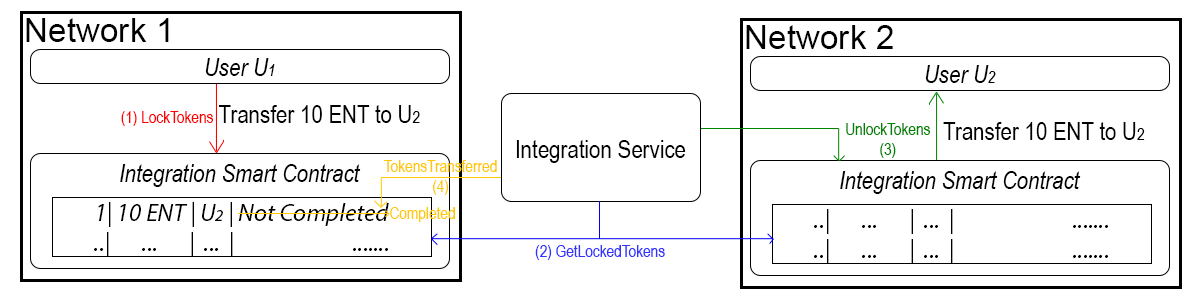
\includegraphics[scale=0.35]{Figures/PowerChain_Integration.png}
    \caption{PowerChain Integration}
\end{figure}
\\ 
The token transfer between the networks happens in the following stages:
\begin{enumerate}
    \item A user $U_1$ in network $A$, wants to send some tokens to user $U_2$ in network $B$
    \item $U_1$ calls the method \textbf{LockTokens} with the public address of $U_2$ as a parameter and sends $X$ amount of tokens.
    \item The integration smart contract of network $A$ locks the tokens in its contract address and stores the public address of $U_2$ along with the amount $X$
    \item The integration service calls method \textbf{GetLockedTokens} of both network $A$ and $B$ every $T$ seconds
    \item The integration service receives the information that $X$ tokens was locked on network $A$ for the public address of $U_2$ and initiates the \textbf{UnlockTokens} method of network $B$
    \item Tokens are unlocked or generated by the integration smart contract of network $B$ and transferred to the public address of $U_2$
    \item The integration service calls the method \textbf{TokensTransferred} of network $A$ to mark the token transfer as complete.
\end{enumerate}
\pagebreak
\section{Summarization}
In this chapter, we analyzed the main limitations we are trying to address with our proposed architecture and then presented all the components of our solution. We went through the information and physical
layers of the architecture and analyzed the network roles and tokens. We discussed in more details about the minting and burning mechanism of the tokens and delve deeper into the blockchain and market layers.
Finally, we proposed a possible integration architecture that could allow the interconnection of multiple energy trading networks that use our proposed solution.